\documentclass[11pt]{article}
\usepackage{float}  % Esto va en el preámbulo
\usepackage[utf8]{inputenc}
\usepackage[spanish]{babel}
\usepackage{graphicx}         % Para incluir imágenes
\usepackage{amsmath}          % Para notación matemática
\usepackage[margin=3cm]{geometry}  % Márgenes
\usepackage[font=normalsize,labelfont=small]{caption}  % Estilo de captions
\usepackage{hyperref}         % Para links clickeables

\documentclass[12pt]{article}

\usepackage[utf8]{inputenc}
\usepackage[spanish]{babel}
\usepackage{graphicx}
\usepackage{amsmath, amssymb}
\usepackage{float}
\usepackage{geometry}
\geometry{a4paper, margin=2.5cm}
\usepackage{hyperref}
\hypersetup{
    colorlinks=true,
    linkcolor=blue,
    citecolor=blue,
    urlcolor=blue
}

\begin{document}

\begin{titlepage}
    \centering
    \vspace*{0.5cm}
    \includegraphics[scale=1.0]{Logo-Udesa.png}\par
    \vspace{10pt}

    {\LARGE \textbf{Fisica II}\par}
    \vspace{1cm}

    {\LARGE \textbf{Trabajo Práctico 1: \\Ley de Ohm y Medición de la Resistencia Interna de un Voltímetro}\par}
    \vspace{2cm}
    
    {\LARGE {Facundo Firpo, Damian  Distefano y Alejo Zimmermann}\par}
    \vspace{4cm}
    
    {\Large \today\par}
    \vspace{1cm}
    \Large{Ingeniería en Inteligencia Artificial}
\end{titlepage}


\begin{abstract}
En esta práctica de laboratorio se llevaron a cabo dos experiencias en el contexto de circuitos eléctricos en corriente continua. La primera consistió en la verificación experimental de la ley de Ohm para un resistor, evaluando la proporcionalidad entre la diferencia de potencial aplicada y la corriente. La segunda experiencia tuvo como objetivo estimar la resistencia interna de un voltímetro, utilizando su efecto en un circuito divisor de tensión.
\end{abstract}

\section*{Introducción}

En esta práctica se abordarán dos experiencias. La primera busca estudiar la relación entre el voltaje, la resistencia y la corriente en un circuito. La segunda experiencia tiene por objetivo determinar la resistencia interna de un voltímetro, utilizando un método basado en un divisor de tensión.

\section*{Marco teórico}

\subsection*{1. Ley de Ohm}

La ley de Ohm, establece que la corriente eléctrica que circula por un conductor es directamente proporcional a la diferencia de potencial aplicada entre sus extremos. Matemáticamente, se expresa como:
\begin{equation}
V = I R
\label{eq:ley-ohm}
\end{equation}
donde \( V \) es la diferencia de potencial (en voltios), \( I \) es la corriente eléctrica (en amperios) y \( R \) es la resistencia del conductor (en ohmios).

\subsection*(2. Propagación de errores)
La propagación de errores es un método utilizado para estimar la incertidumbre en una medición derivada de otras mediciones. En este caso, se aplicará la regla de propagación de errores para calcular la incertidumbre en la resistencia interna del voltímetro, que se obtiene a partir de la ecuación \ref{eq:resistencia-interna}.
La resistencia interna del voltímetro \( R_V \) se determina a partir de la relación:

\begin{equation}
R_V = \frac{R}{\frac{E_0}{V_V} - 1}
\label{eq:resistencia-interna}
\end{equation}
donde \( R \) es la resistencia del divisor de tensión, \( E_0 \) es el voltaje de la fuente y \( V_V \) es el voltaje medido por el voltímetro. La incertidumbre en \( R_V \) se puede calcular utilizando la regla de propagación de errores:
\begin{equation}
\Delta R_V = R_V \sqrt{\left(\frac{\Delta R}{R}\right)^2 + \left(\frac{\Delta E_0}{E_0}\right)^2 + \left(\frac{\Delta V_V}{V_V}\right)^2}
\label{eq:propagacion}
\end{equation}
donde \( \Delta R \), \( \Delta E_0 \) y \( \Delta V_V \) son las incertidumbres asociadas a las mediciones de \( R \), \( E_0 \) y \( V_V \) respectivamente. Esta ecuación permite estimar la incertidumbre en la resistencia interna del voltímetro teniendo en cuenta las incertidumbres de las mediciones involucradas.

\section*{Resumen de experiencias}
En este trabajo, se aplicaron los conceptos del marco teórico para verificar experimentalmente la ley de Ohm y para estimar la resistencia interna de un voltímetro. Todas las mediciones fueron tomadas con multímetros utilizados como voltímetros y amperímetros.

\subsection*{1. Verificación de la Ley de Ohm}

Se estudia la relación entre la diferencia de potencial aplicada a una resistencia y la corriente que circula por ella. De acuerdo con la ley de Ohm, se espera una relación lineal como la de la ecuación \ref{eq:ley-ohm}. Se armó un circuito simple con una fuente variable, un resistor y un amperímetro para medir la corriente.

\begin{figure}[H]
    \centering
    \includegraphics[width=0.5\linewidth]{ej1.png}
    \caption{Circuito armado para evaluar la Ley de Ohm donde E es el voltaje de la fuente, i es la corriente dada por la fuente, V es el voltímetro, A es el amperímetro y la X la resistencia.}
    \label{fig:ej1}
\end{figure}

En las mediciones utilizamos dos resistencias distintas, una de $9.6k\Omega$ y otra de $98k\Omega$, para cada uno de ellas variamos el voltaje emitido por la fuente entre $0.5V$ y $5V$. Con estos datos se logró construir un ajuste lineal y verificar si efectivamente se cumple la Ley de Ohm. 

Para tomar las mediciones, como se puede observar en la figura \ref{fig:ej1}, se utilizó un voltímetro en paralelo con la resistencia y un amperímetro en serie con la resistencia. El voltímetro estaba en paralelo para medir la caída de potencial al pasar por la resistencia mientras que el amperímetro en serie media la corriente. Durante las mediciones, se consideró que las mediciones de los multímetros eran más certeras que las de la fuente directa. Durante el experimento se evitaron voltajes elevados para proteger los equipamientos.

\subsection*{2. Medición de la resistencia interna del voltímetro}

Se utilizó un divisor de tensión como visto en \ref{fig:ej2} formado por una resistencia variable \( R \) y el voltímetro, cuya resistencia interna \( R_V \) se desea determinar. A partir de la Ley de Ohm \ref{eq:ley-ohm}, conseguimos la relación:

\begin{equation*}
    V_V = I \cdot R_V
\end{equation*}

\begin{equation*}
    E_0 = I \cdot (R + R_V)
\end{equation*}

\begin{equation}
    R_V = \frac{R}{\frac{E_0}{V_V} - 1}
    \label{eq:resistencia-interna}
\end{equation}

donde $E_0$ es el voltaje de la fuente, y $V_V$ es el voltaje medido por el voltímetro.

Se varió el valor de R en tres ocasiones, $9.6k\Omega$, $98k\Omega$ y $990k\Omega$. Para cada una se evaluaron $E_0$ de entre $9V$ y $17V$.

El sistema de armó de la siguiente forma:

\begin{figure}[H]
    \centering
    \includegraphics[width=0.5\linewidth]{ej2.png}
    \caption{Circuito armado para evaluar la resistencia del voltímetro donde $E_0$ es el voltaje de la fuente, R es la resistencia, V es el voltaje medido por el voltímetro y $R_V$ es la resistencia del voltímetro}
    \label{fig:ej2}
\end{figure}

\section*{Mediciones}

\subsection*{1. Fuente}

Esta permite variar el voltaje de salida manualmente mediante perillas y visualizar su valor en una pantalla digital. Se utilizó para aplicar distintas diferencias de potencial sobre el resistor bajo estudio y también para alimentar el divisor de tensión en la segunda experiencia.

La fuente que se utilizó podía proporcionar un máximo de $5A$ y $30V$. La medición del amperaje de la fuente tenia una incerteza del $\pm 0.01$ mientras que la medición del voltaje de la fuente tenia una incerteza del $\pm 0.1$.

\subsection*{2. Multímetro}

El multímetro digital empleado permite realizar mediciones de voltaje, corriente y resistencia. En esta práctica, se utilizó principalmente para medir la tensión en distintos puntos del circuito, así como también para medir la corriente mediante la inserción en serie. Dado que el multímetro no es ideal y posee una resistencia interna finita, se analizó su influencia en el circuito divisor de tensión.

Para obtener un mejor conocimiento del comportamiento del multímetro, se comparó el voltaje que este mide con el voltaje entregado por la fuente. Como se puede ver en la figura \ref{fig:vvsf} la relación es lineal. Esta comparación permite calibrar el sistema y determinar la relación entre el valor medido y el valor aplicado.

\begin{figure}[H]
    \centering
    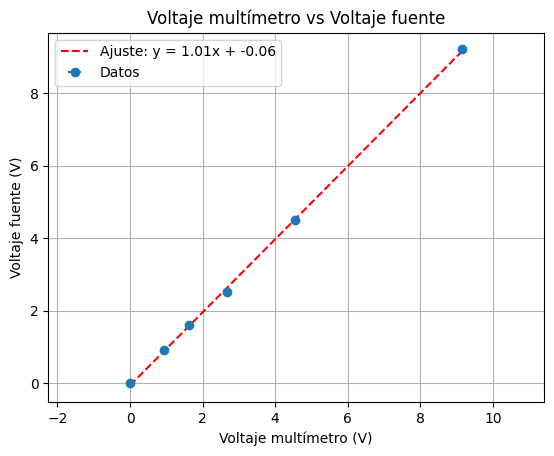
\includegraphics[width=.9\linewidth]{VvsV.png}
    \caption{Voltaje medido por el multímetro vs voltaje suministrado por la fuente. El $V_m$ tiene una incerteza de $\pm 0.01V$ y $V_f$ de $\pm0.1V$.}
    \label{fig:VvsV}
\end{figure}

\section*{Resultados}

\subsection*{1. Experiencia 1}

En esta experiencia se verificó la ley de Ohm. Se midió con el voltímetro la caída del potencial y con el amperímetro la corriente. Luego se representaron gráficamente los datos, realizando un ajuste lineal, observando una clara relación lineal entre tensión y corriente. La pendiente de cada recta obtenida representa la resistencia del componente.

\begin{figure}[H]
    \centering
    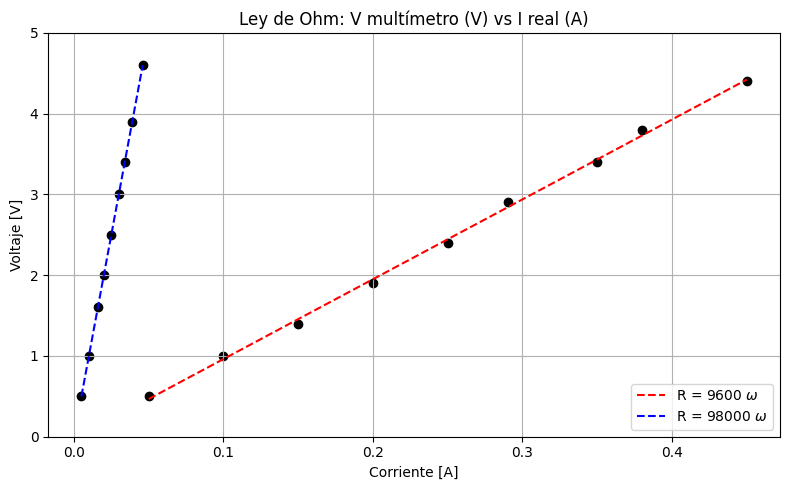
\includegraphics[width=0.8\linewidth]{Ohm.png}
    \caption{Gráfico de diferencia de voltaje medido por el voltímetro vs corriente medida por el amperímetro para dos resistores distintos. Las pendientes indican los valores de resistencia obtenidos experimentalmente. Tanto el voltaje como la corriente fueron medidos con una incerteza de $\pm 0.01$ V y A respectivamente.}
    \label{fig:ohm}
\end{figure}

\subsection*{2. Experiencia 2}

En esta segunda experiencia se analizó el efecto del multímetro sobre un circuito divisor de tensión. Se construyó un divisor utilizando dos resistores en serie, y se midió el voltaje sobre uno de ellos con el multímetro. Como el instrumento tiene resistencia interna finita, introduce una carga en el circuito, modificando el valor de la tensión medida. A partir de esta perturbación y aplicando las leyes de circuitos, se estimó la resistencia interna del multímetro.

\begin{table}[h]
    \centering
    \begin{tabular}{|c|c|c|c|c|}
        \hline
        $R$ [$k\Omega$]  & $V_V \pm 0.01$ [V] & $E_0 \pm 0.1$ [V] & $R_V$ [$M\Omega$] & $\Delta R_V$ [$M\Omega$] \\ \hline
        9.6   & 10.3   & 10.5   & 0.49   & 0.25 \\ \hline
        9.6   & 13.1   & 13.4   & 0.42   & 0.14 \\ \hline
        9.6   & 15.6   & 15.8   & 0.75   & 0.38 \\ \hline
        98    & 13.4   & 13.7   & 4.38   & 1.47 \\ \hline
        98    & 16.8   & 17.1   & 5.49   & 1.84 \\ \hline
        990   & 8.33   & 9.2    & 9.48   & 5.27 \\ \hline
        990   & 11.62  & 12.8   & 9.75   & 3.77 \\ \hline
        990   & 13.34  & 14.6   & 10.48  & 3.54 \\ \hline
    \end{tabular}
    \caption{Placeholder caption for a table with 9 rows and 5 columns.}
    \label{tab:placeholder_label}
\end{table}

\section*{Conclusiones}



En la primera experiencia, se logró verificar experimentalmente la ley de Ohm. Los gráficos obtenidos mostraron una relación lineal clara entre la diferencia de potencial y la corriente, lo cual confirma la proporcionalidad establecida por dicha ley. Las pendientes de las rectas obtenidas permitieron calcular resistencias que resultaron coherentes con los valores esperados. Esta experiencia puso en evidencia la utilidad de los métodos gráficos para determinar parámetros eléctricos de manera sencilla y precisa.

En la segunda experiencia, se observó cómo la resistencia interna del voltímetro influye en las mediciones de tensión en un circuito divisor. A través de un análisis teórico-experimental, se pudo estimar el valor de dicha resistencia interna, evidenciando que los instrumentos de medición no son ideales y pueden perturbar el sistema que intentan medir. Esta situación es especialmente importante cuando se trabaja con resistencias de valores elevados, ya que la carga introducida por el instrumento puede afectar significativamente el resultado.


\end{document}
